\documentclass[fleqn,10pt,french]{SelfArx} % Document font size and equations flushed left

\usepackage{lipsum} % Required to insert dummy text. To be removed otherwise
\usepackage[utf8]{inputenc} 
\usepackage{multirow}
\usepackage{booktabs}
\usepackage{threeparttable}
\usepackage{colortbl}
\usepackage{xcolor}

\setlength{\parindent}{10pt}

\usepackage{caption}
\captionsetup[table]{name=Tableau}

\setlength{\columnsep}{0.55cm} % Distance between the two columns of text
\setlength{\fboxrule}{0.75pt} % Width of the border around the abstract

\definecolor{color1}{RGB}{0,0,90} % Color of the article title and sections
\definecolor{color2}{RGB}{0,20,20} % Color of the boxes behind the abstract and headings

\usepackage{hyperref} 
\hypersetup{hidelinks,colorlinks,breaklinks=true,urlcolor=color2,citecolor=color1,linkcolor=color1,bookmarksopen=false,pdftitle={Title},pdfauthor={Author}}

\Archive{Projet d’INF 421} 
\PaperTitle{Résoudre de manière optimale le Rubik’s cube} 
\Authors{Kevin CHEN, Yuxiang LI} 
\affiliation{*\textbf{Code source}: https://github.com/lyx-x/Rubik} 
\Keywords{IDA* --- Pattern Database --- HashMap}
\newcommand{\keywordname}{Keywords}

%----------------------------------------------------------------------------------------
%	ABSTRACT
%----------------------------------------------------------------------------------------

\Abstract{TODO}

%----------------------------------------------------------------------------------------

\begin{document}

\flushbottom % Makes all text pages the same height

\maketitle % Print the title and abstract box

\renewcommand{\contentsname}{Table des matières}
\tableofcontents % Print the contents section

\thispagestyle{empty} % Removes page numbering from the first page

%----------------------------------------------------------------------------------------
%	ARTICLE CONTENTS
%----------------------------------------------------------------------------------------

\section{Analyse du sujet} % The \section*{} command stops section numbering

\lipsum[1-3] % Dummy text
 and some mathematics $\cos\pi=-1$ and $\alpha$ in the text\footnote{And some mathematics $\cos\pi=-1$ and $\alpha$ in the text.}.

%------------------------------------------------

\section{Implémentation}

\begin{figure*}[ht]\centering % Using \begin{figure*} makes the figure take up the entire width of the page
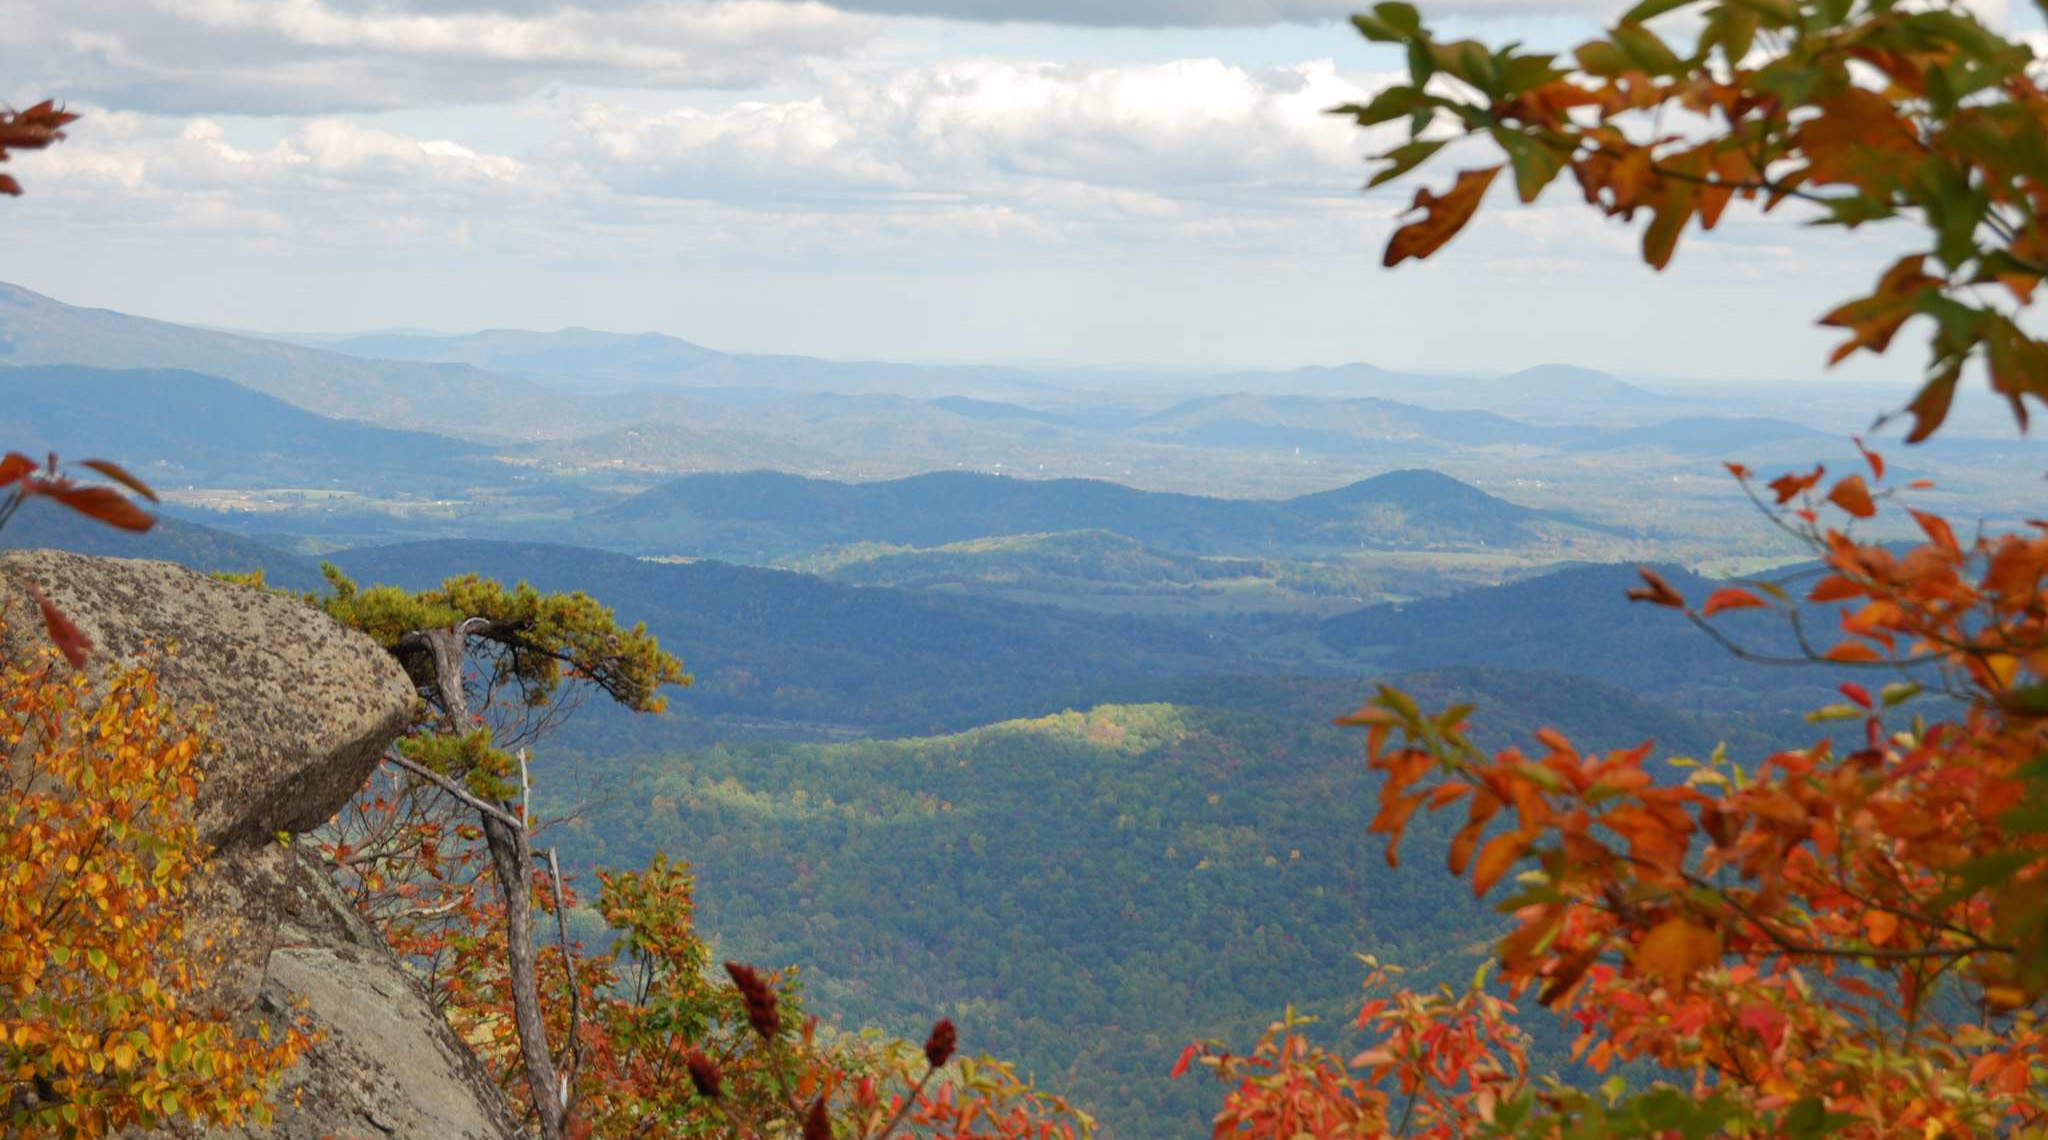
\includegraphics[width=\linewidth]{view}
\caption{Wide Picture}
\label{fig:view}
\end{figure*}

\lipsum[4] % Dummy text

\begin{equation}
\cos^3 \theta =\frac{1}{4}\cos\theta+\frac{3}{4}\cos 3\theta
\label{eq:refname2}
\end{equation}

\lipsum[5] % Dummy text

\begin{enumerate}[noitemsep] % [noitemsep] removes whitespace between the items for a compact look
\item First item in a list
\item Second item in a list
\item Third item in a list
\end{enumerate}

\subsection{Organisation du code}

\lipsum[6] % Dummy text

\paragraph{Paragraph} \lipsum[7] % Dummy text
\paragraph{Paragraph} \lipsum[8] % Dummy text

\subsection{Algorithmes de recherche}

\lipsum[9] % Dummy text

\begin{figure}[ht]\centering
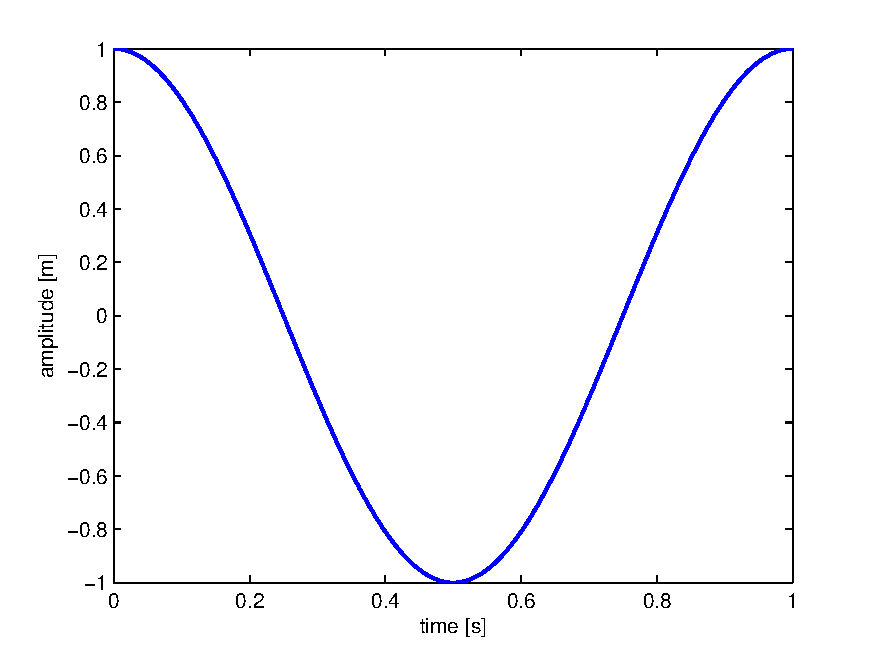
\includegraphics[width=\linewidth]{results}
\caption{In-text Picture}
\label{fig:results}
\end{figure}

Reference to Figure \ref{fig:results}.

%------------------------------------------------

\section{Résultats}

\lipsum[10] % Dummy text

\subsection{Tests}

\lipsum[11] % Dummy text

\subsection{Problèmes rencontrés}

\lipsum[11] % Dummy text

\begin{table}[hbt]
\caption{Table of Grades}
\centering
\begin{tabular}{llr}
\toprule
\multicolumn{2}{c}{Name} \\
\cmidrule(r){1-2}
First name & Last Name & Grade \\
\midrule
John & Doe & $7.5$ \\
Richard & Miles & $2$ \\
\bottomrule
\end{tabular}
\label{tab:label}
\end{table}

\subsubsection{Estimateur de la distance}

\lipsum[12] % Dummy text

\subsubsection{HashCode}

\lipsum[12] % Dummy text

\subsubsection{Opération du fichier}

\lipsum[12] % Dummy text

\begin{description}
\item[Word] Definition
\item[Concept] Explanation
\item[Idea] Text
\end{description}

\subsubsection{Pattern database}

\lipsum[13] % Dummy text

\subsubsection{Taille de HashMap}

\lipsum[13] % Dummy text

\begin{itemize}[noitemsep] % [noitemsep] removes whitespace between the items for a compact look
\item First item in a list
\item Second item in a list
\item Third item in a list
\end{itemize}

\subsection{Comparaison et conclusion}

Plus un programme est lord, plus on sent l’importance des algorithmes et des structures de données. La résolution de Rubik’s Cube, faisant partie de cette catégorie de programmes, nous a fait beaucoup réfléchi sur les algorithmes que nous utilisons afin d’aller plus loin dans la recherche de solution. Nous avons constaté au cours du temps qu’à chaque modification majeure du code, le programme devient plus rapide. Au début, le programme ne pouvait trouver que des solutions à 5 étapes avec une recherche naîve, puis le nombre d’étapes est passé à 7 même 8 en implémentant IDA*, à la fin ce record a été battu par une solution à 13 étapes en 42 secondes après avoir étudié plus de 900 000 cas possibles. 

\subsubsection{Algorithmes de recherche}

Dans la section précédente, nous avons présenté les 3 algorithms testés. Pour se donner une idée de la performance de chaque algorithme, on pourra jeter un coup d’oeil sur le résultat d’un test de comparaison entre les différentes méthodes. 

\begin{table}[htbp]
\centering
\begin{tabular}{cccc}
\hline
\rowcolor{blue!20} \rule{0pt}{12pt} \textbf{Profondeur} & \textbf{DFS\textsuperscript{1} (PQ)\textsuperscript{2}} & \textbf{DFS}\textsuperscript{1} & \textbf{IDA*}\\
\hline
1 & 0 & 0 & 0  \\
%\hline
2 & 0 & 0 & 0 \\
%\hline
3 & 0 & 1 & 0 \\
%\hline
4 & 17 & 7 & 0 \\
%\hline
5 & 387 & 246 & 0 \\
%\hline
6 & (48865)\textsuperscript{3} & (27989)\textsuperscript{3} & 0  \\
%\hline
7 & - & - & 0 \\
%\hline
8 & - & - & 2 \\
%\hline
9 & - & - & 7 \\
%\hline
10 & - & - & 87 \\
%\hline
11 & - & - & 1143 \\
%\hline
12 & - & - & 5270 \\
%\hline
13 & - & - & (31488)\textsuperscript{3} \\
%\hline
14 & - & - & - \\
\hline
\multicolumn{4}{l}{\small{1. DFS avec une profondeur limité}} \\
\multicolumn{4}{l}{\small{2. Ce parcours utilise une queue de priorité}} \\
\multicolumn{4}{l}{\small{3. Cette valeur est calculée avec moins de 5 essais}} \\
\hline
~\\
\end{tabular}
\caption{Temps moyens de la recherche (algorithme)}
\end{table}

\indent
On constate que l’utilisation de la queue de priorité n’a pas amélioré la vitesse de recherche, ce qui est dû principalement à la maintenance de la queue, car une recherche en profondeur avec la limite de profondeur qui s’incrément un par un ne se diffère pas vraiment d’un parcours en largeur. Dans ce cas-là, l’utilisation de la queue de priorité n’est pas rentable, parce qu’on finit toujours pas parcourir presque toutes les configurations. On pourrait penser à utiliser une queue de priorité afin d’implémenter un parcours A*, mais cette méthode ne donne pas un chemin minimal dans la plupart des cas. Comme une solution manuelle de Robik’s Cube existe déjà, la seule question qui reste aujourd’hui est de savoir comment la résoudre d’une manière optimale.

Quant à l’algorithme IDA*, ce résultat n’est point surprenant. Pour une solution de moins de 6 étapes (ce qui correspond au niveau de notre Pattern Database, c’est-à-dire qu’il possède toutes les configurations d’une distance inférieure ou égale à 6), à chaque appel récursif, on est sûr de s’approcher de l’état final, ceci dit qu’on a toujours au moins un chemin pour faire diminuer la distance. Et comme la distance initiale est inférieure ou égale à 6, la solution sera trouvé immédiatement. Au-delà de 6 étapes, on constate qu’il y a une augmentation de temps comme dans les autres cas, cela vient du fait qu’on ne peut pas distinguer par exemple une distance 10 et une distance 7 à cause de la taille de notre base de données, cela brouille la piste de recherche et on est obligé d’étudier beaucoup de cas comme s’ils étaient de la même distance. On pourrait comprendre cet algorithme comme une translation (sur l’axe de profondeur) d’une distance imposée par le niveau de Pattern Database.

\subsubsection{Estimateurs de distance} 

Pour utiliser l’algorithme IDA*, il nous faut une fonction heuristique ou un estimateur de distance. Les conditions nécessaires et suffisantes d’utilisation d’une telle fonction sont prouvées dans la section précédente. Ici, on va comparer de diverses fonctions et essayer de comprendre en quoi elles sont différentes. 

\begin{table}[htbp]
\centering
\begin{tabular}{cccc}
\hline
\rowcolor{blue!20} \rule{0pt}{12pt} \textbf{Profondeur} & \textbf{Simple\textsuperscript{1} } & \textbf{Manhattan}\textsuperscript{1} & \textbf{Pattern\textsuperscript{1}}\\
\hline
3 & 0 & 3 & 0 \\
4 & 2 & 5 & 0 \\
5 & 20 & 26 & 0 \\
6 & 223 & 135 & 0  \\
7 & 1380 & 215 & 0 \\
8 & - & 1118 & 1 \\
9 & - & - & 13 \\
10 & - & - & 79 \\
11 & - & - & 1161 \\
12 & - & - & 7309 \\
\hline
\multicolumn{4}{l}{\small{1. Le calcul se trouve dans la section précédente}} \\
\hline
~\\
\end{tabular}
\caption{Temps moyens de la recherche (estimateur)}
\end{table}

\begin{table}[htbp]
\centering
\begin{tabular}{cccc}
\hline
\rowcolor{blue!20} \rule{0pt}{12pt} \textbf{Profondeur} & \textbf{Coins\textsuperscript{1} } & \textbf{Arêtes 1}\textsuperscript{1} & \textbf{Arêtes 2\textsuperscript{1}}\\
\hline
4 & 0 & 0 & 2 \\
5 & 2 & 0 & 90 \\
6 & 8 & 0 & 220  \\
7 & 38 & 1 & 1256 \\
8 & 123 & 13 & - \\
9 & 220 & 144 & - \\
10 & 1855 & 339 & - \\
11 & - & 1108 & - \\
\hline
\multicolumn{4}{l}{\small{1. Le calcul se trouve dans la section précédente}} \\
\hline
~\\
\end{tabular}
\caption{Temps moyens de la recherche (Pattern)}
\end{table}

\subsubsection{Conclusion}

Bien que le résultat précédent n’est pas suffisant pour résoudre un cube quelconque, il nous donne une piste de l’amélioration : agrandir Pattern Database et améliorer HashMap et HashCode. Plus la base de données est large, plus on choisit la bonne direction. Et puis le deuxième intervient lors de l’éxécution du programme, car la taille de HashMap est limité par l’environnement de JVM et cette taille va déterminer la vitesse de la recherche. Rien n’interdit de résoudre complètement le Rubik’s Cube, mais cela demandera une recherche encore plus poussée que les analyses dans ce rapport et surtout un ordinateur plus puissant.

%------------------------------------------------
\phantomsection
\section*{Annexe} % The \section*{} command stops section numbering

\addcontentsline{toc}{section}{Annexe} % Adds this section to the table of contents

So long and thanks for all the fish \cite{Figueredo:2009dg}.

\end{document}